\newpage
\hypertarget{allCards vis}{}
\section{AllOtherPartitionsRule}
\genHeader

\begin{stepbystep}

\item Create a new rule \texttt{AllOtherPartitionsRule}, and complete it according to \Cref{fig:ea_AllOtherPartitionsRuleComplete}.


\begin{figure}[htbp]
\begin{center}
  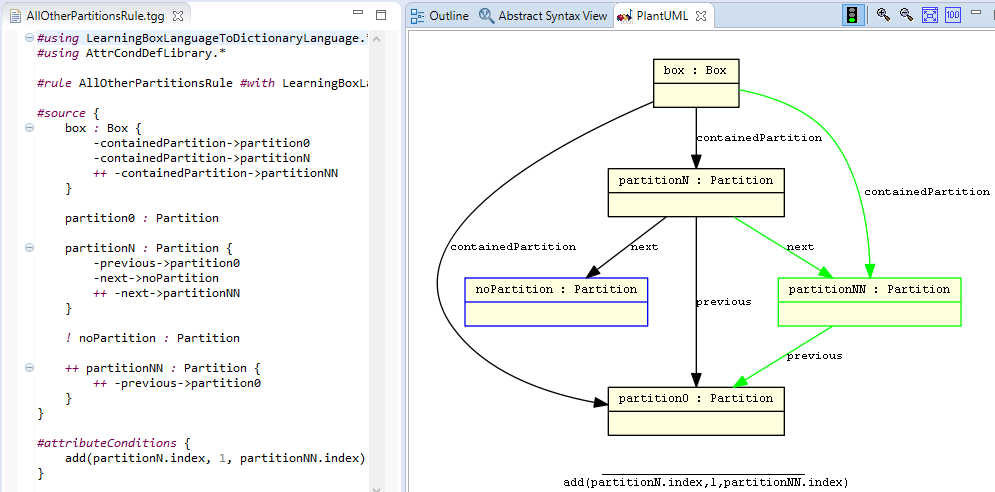
\includegraphics[width=\textwidth]{../../org.moflon.doc.handbook.04_tripleGraphTransformations/6_extendingTransformation/visProtoImages/ea_AllOtherPartitionsRule}
  \caption{The completed \texttt{AllOtherPartitionsRule}}
  \label{fig:ea_AllOtherPartitionsRuleComplete}
\end{center}
\end{figure}

\item As you can see, this rule doesn't assume to know the final \texttt{partition} in the transformation. 
It matches the \texttt{n}th partition as the partition without any next partition, then connects a new $(n+1)$-th partition to the $n$ partition and \moslTggCode{partition0} (clear as every partitions previous is \moslTggCode{partition0}).
Note that TGG transformations assume that the models are valid, \idest, have the expected structure (in our case meaning that the learning box is correctly \enquote{wired}).\footnote{This should actually be formalised with a set of metamodel constraints that must be checked before a transformation is run, but we've omitted this here to simplify things.}  
Remember that \enquote{blue} means \enquote{negative}.

\item Re-run the transformation after the code for your improved TGG has been generated. 
It should work now without any error message.
Inspect the protocol to understand what happened.

\item Go ahead and add as many \moslTggCode{Partitions} and \moslTggCode{Card} as you like to your model instance.
Your TGG is now also able to handle a \moslTggCode{Box} with any number of \moslTggCode{Partitions} beautifully.
For five partitions all with cards, the protocol gets quite interesting and is no longer a flat tree.
Try it out! 

\end{stepbystep}
